\documentclass{article}[18pt]
\ProvidesPackage{format}
%Page setup
\usepackage[utf8]{inputenc}
\usepackage[margin=0.7in]{geometry}
\usepackage{parselines} 
\usepackage[english]{babel}
\usepackage{fancyhdr}
\usepackage{titlesec}
\hyphenpenalty=10000

\pagestyle{fancy}
\fancyhf{}
\rhead{Sam Robbins}
\rfoot{Page \thepage}

%Characters
\usepackage{amsmath}
\usepackage{amssymb}
\usepackage{gensymb}
\newcommand{\R}{\mathbb{R}}

%Diagrams
\usepackage{pgfplots}
\usepackage{graphicx}
\usepackage{tabularx}
\usepackage{relsize}
\pgfplotsset{width=10cm,compat=1.9}
\usepackage{float}

%Length Setting
\titlespacing\section{0pt}{14pt plus 4pt minus 2pt}{0pt plus 2pt minus 2pt}
\newlength\tindent
\setlength{\tindent}{\parindent}
\setlength{\parindent}{0pt}
\renewcommand{\indent}{\hspace*{\tindent}}

%Programming Font
\usepackage{courier}
\usepackage{listings}
\usepackage{pxfonts}

%Lists
\usepackage{enumerate}
\usepackage{enumitem}

% Networks Macro
\usepackage{tikz}


% Commands for files converted using pandoc
\providecommand{\tightlist}{%
	\setlength{\itemsep}{0pt}\setlength{\parskip}{0pt}}
\usepackage{hyperref}

% Get nice commands for floor and ceil
\usepackage{mathtools}
\DeclarePairedDelimiter{\ceil}{\lceil}{\rceil}
\DeclarePairedDelimiter{\floor}{\lfloor}{\rfloor}

% Allow itemize to go up to 20 levels deep (just change the number if you need more you madman)
\usepackage{enumitem}
\setlistdepth{20}
\renewlist{itemize}{itemize}{20}

% initially, use dots for all levels
\setlist[itemize]{label=$\cdot$}

% customize the first 3 levels
\setlist[itemize,1]{label=\textbullet}
\setlist[itemize,2]{label=--}
\setlist[itemize,3]{label=*}

% Definition and Important Stuff
% Important stuff
\usepackage[framemethod=TikZ]{mdframed}

\newcounter{theo}[section]\setcounter{theo}{0}
\renewcommand{\thetheo}{\arabic{section}.\arabic{theo}}
\newenvironment{important}[1][]{%
	\refstepcounter{theo}%
	\ifstrempty{#1}%
	{\mdfsetup{%
			frametitle={%
				\tikz[baseline=(current bounding box.east),outer sep=0pt]
				\node[anchor=east,rectangle,fill=red!50]
				{\strut Important};}}
	}%
	{\mdfsetup{%
			frametitle={%
				\tikz[baseline=(current bounding box.east),outer sep=0pt]
				\node[anchor=east,rectangle,fill=red!50]
				{\strut Important:~#1};}}%
	}%
	\mdfsetup{innertopmargin=10pt,linecolor=red!50,%
		linewidth=2pt,topline=true,%
		frametitleaboveskip=\dimexpr-\ht\strutbox\relax
	}
	\begin{mdframed}[]\relax%
		\centering
		}{\end{mdframed}}



\newcounter{lem}[section]\setcounter{lem}{0}
\renewcommand{\thelem}{\arabic{section}.\arabic{lem}}
\newenvironment{defin}[1][]{%
	\refstepcounter{lem}%
	\ifstrempty{#1}%
	{\mdfsetup{%
			frametitle={%
				\tikz[baseline=(current bounding box.east),outer sep=0pt]
				\node[anchor=east,rectangle,fill=blue!20]
				{\strut Definition};}}
	}%
	{\mdfsetup{%
			frametitle={%
				\tikz[baseline=(current bounding box.east),outer sep=0pt]
				\node[anchor=east,rectangle,fill=blue!20]
				{\strut Definition:~#1};}}%
	}%
	\mdfsetup{innertopmargin=10pt,linecolor=blue!20,%
		linewidth=2pt,topline=true,%
		frametitleaboveskip=\dimexpr-\ht\strutbox\relax
	}
	\begin{mdframed}[]\relax%
		\centering
		}{\end{mdframed}}
\lhead{MCS - LDS}


\begin{document}
\begin{center}
\underline{\huge Prenex Normal Form}
\end{center}
\section{Logical equivalence}
Recall that two formula $\phi$ and $\psi$ are logically equivalent if they are true for the same set of models, in which case we write
$$\phi\equiv\psi$$
\section{Parse Trees}
Recall that to check if a formula is well formed we can use a parse tree. We illustrated this with
\begin{center}
	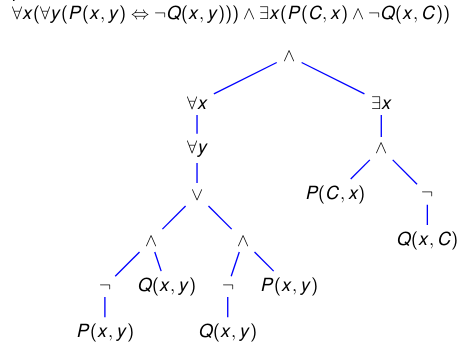
\includegraphics[scale=0.7]{parse}
\end{center}
\section{Prenex Normal Form}
We are not in a position to obtain an important normal form. Consider the process of constructing a forst order formula: We start from atoms and construct increasingly more complex formula using $\land,\lor,\lnot,\exists$ and $\forall$, with a structure of a formula given by its parse tree.\\
We say that a first order formula is in prenex normal form if it is written in the form
$$Q _ { 1 } x _ { 1 } Q _ { 2 } x _ { 2 } \ldots Q _ { k } x _ { k } \phi$$
Where:
\begin{itemize}
	\item each $Q_i$ is a quantifier
	\item each $x_i$ is a variable
	\item the formula $\phi$ is quantifier free (so all the logic symbols like $\land$ are in here)
\end{itemize}
We shall show that every first order formula is equivalent to one in prenex normal form
\section{Establishing prenex normal form}
We use the parse tree of a formula $\phi$ in order to construct an equivalent formula in prenex normal form.\\
\\
A key observation is that if we choose some node of the parse tree of $\phi$ and look at the sub-tree with this node as root then this subtree corresponds to a sub formula of $\phi$, that is, to a formula apprearing as a formula within $\phi$\\
\\
What we do is start at the leaves of the parse tree and work up the tree repeatedly constructing prenex normal form formulae that are equivalent to the formulae corresponding to sub-trees of the parse tree\\
\\
Let's start at the leaves. The formula at each leaf is trivially in prenex normal form (as it involves no quantifiers)\\
\\
Suppose that we have reached a node of the parse tree that is a $\land$-node and that we have constructed prenex normal form formulae equivalent to the formulae corresponding to the subtrees rooted at the 2 children of this $\land$-node\\
\\
So, the formula corresponding to the subtree rooted at this $\land$-node is of the form $\psi\land \chi$ and we have already constructed $\psi'$ and $\chi'$ such that:
\begin{itemize}
	\item $\psi'$ and $\chi'$ are in prenex normal form:
	\begin{itemize}
		\item $\psi'$ is $Q _ { 1 } x _ { 1 } Q _ { 2 } x _ { 2 } \cdots Q _ { k } x _ { k } \psi ^ { \prime \prime }$ quantifier tree (and each $Q_i$ a quantifier)
		\item $\chi'$ is $P _ { 1 } y _ { 1 } P _ { 2 } y _ { 2 } \cdots P _ { k } y _ { k } \chi ^ { \prime \prime }$ with $\chi ^ { \prime \prime }$ quantifier free (and each $P_i$ a quantifier)
	\end{itemize}
	\item $\psi\equiv\psi'$
	\item $\chi\equiv\chi'$
\end{itemize}
Note that by renaming bound variables (if necessary) we may assume that no $x_i$ is the same variable as any $y_j$\\
So $\psi\land \chi$ is equivalent to a formula in prenex normal form
$$\begin{aligned} \psi \wedge \chi & \equiv Q _ { 1 } x _ { 1 } Q _ { 2 } x _ { 2 } \cdots Q _ { k } x _ { k } \psi ^ { \prime \prime } \wedge P _ { 1 } y _ { 1 } P _ { 2 } y _ { 2 } \cdots P _ { k } y _ { k } \chi ^ { \prime \prime } \\ & \equiv Q _ { 1 } x _ { 1 } Q _ { 2 } x _ { 2 } \cdots Q _ { k } x _ { k } P _ { 1 } y _ { 1 } P _ { 2 } y _ { 2 } \cdots P _ { k } y _ { k } \left( \psi ^ { \prime \prime } \wedge \chi ^ { \prime \prime } \right) \end{aligned}$$
The same construction works for a $\land$ node of our parse tree.\\
Consider a $\lnot$ node\\
Now we have that the formula corresponding to the sub tree rooted at this $\lnot$ node is equivalent to a formula of the form $Q _ { 1 } x _ { 1 } Q _ { 2 } x _ { 2 } \cdots Q _ { k } x _ { k } \psi ^ { \prime \prime }$ with $\psi''$ quantifier free (and each $Q_i$ a quatifier).\\
Hence, using our general rule from earlier, this formula is equivalent to $Q _ { 1 } x _ { 1 } Q _ { 2 } x _ { 2 } \cdots Q _ { k } x _ { k } \neg \psi ^ { \prime \prime }$ which is in prenex normal form.\\
\\
Consider a $\forall$ node.\\
Now we have that the formula corresponding to the sub-tree rooted at this $\forall$ node is equivalent to a formula of the form: $Q _ { 1 } x _ { 1 } Q _ { 2 } x _ { 2 } \cdots Q _ { k } x _ { k } \psi ^ { \prime \prime }$ with $\psi''$ quantifier free (and each $Q_i$ a quantifier)\\
However, this is immediately in prenex normal form (the same construction works for a $\exists$ node of our parse tree)\\
Hence, continuing in this way yields an equivalent formula to $\phi$ in prenex normal form
\end{document}